\documentclass[11pt, titlepage, openany]{ltjsbook}
%二段組にするなら[, twocolumn]

% =========================
% 数学
% =========================
\usepackage{amsmath}
\usepackage{amssymb}
\usepackage{mathtools}
\usepackage{bm}
\usepackage{cases}
\usepackage{physics}
\usepackage{siunitx}

% =========================
% 図・色
% =========================
\usepackage{graphicx}
\usepackage{xcolor}
\usepackage{float}
\usepackage{subcaption}
\usepackage{wrapfig}
\usepackage{caption}

% =========================
% TikZ
% =========================
\usepackage{tikz}
\usepackage{tikz-3dplot}
\usetikzlibrary{math}
\usetikzlibrary{arrows.meta}
\usetikzlibrary{calc}
\usetikzlibrary{patterns.meta}
\usetikzlibrary{intersections}
\usetikzlibrary{backgrounds}
\pgfdeclarelayer{background}
\pgfsetlayers{background,main}


% =========================
% 枠・装飾
% =========================
\usepackage[framemethod=tikz]{mdframed}
\usepackage{fancybox}
\usepackage{ascmac}
\usepackage{diagbox}
\newcommand{\slashcell}{\diagbox[width=3.5em,height=2em]{}{}}


% =========================
% レイアウト
% =========================
\usepackage[top=20mm, bottom=20mm, left=20mm, right=20mm]{geometry}
\usepackage{nidanfloat}
\usepackage{enumitem}
\usepackage{varwidth}

% =========================
% 日本語
% =========================
\usepackage{luatexja}
\usepackage{luatexja-fontspec}
%\usepackage[deluxe]{otf}

% =========================
% コード表示
% =========================
\usepackage{listings}
\usepackage{jvlisting}
\usepackage{xcolor}
\usepackage{minted}

\definecolor{codebg}{RGB}{246,249,251}
\definecolor{coderule}{RGB}{176,190,205}
\usemintedstyle{pastie}
\setminted{
  linenos,
  breaklines,
  breakanywhere,
  fontsize=\scriptsize,
  frame=single,
  framesep=2mm,
  baselinestretch=1.0,
  bgcolor=codebg,
  rulecolor=coderule,
  tabsize=2,
  numbersep=6pt,
}

% =========================
% その他
% =========================
\usepackage{url}
\usepackage{hyperref}
\usepackage{appendix}
\setcounter{tocdepth}{2}


% =========================
% タイトル
% =========================
\title{\huge{物質の電気伝導と物性}}
\author{\vspace{3cm}\\
\Large{担当教員}\\
\vspace{2cm}\Large{蒋先生}\\
\Large{04B24032}\\
\Large{笹伶夷}\\
\vspace{2cm}\Large{共同実験者：田處}\\
\Large{実験日：2026年6月23日、6月24日、6月20日、7月1日}
}
\date{}

\begin{document}
\maketitle
\tableofcontents
\clearpage

\chapter{はじめに}
%1.1
\section{概要}
%1.2
\section{理論}
\subsection{金属}
結晶を構成する原子が規則正しく並んでいる場合、その周期ポテンシャルは電子の散乱の原因とはならず、伝導電子は有効質量$m^{*}$を持つ自由電子として振る舞う。
電子が不純物や格子振動から受ける散乱を、速度に比例した抵抗力$-m^{*}v/\tau$と考える。電子に一様電場$E$をかけたときの運動方程式は、
\begin{equation}
  m^{*} \frac{dv}{dt} = -eE -\frac{m^{*}}{\tau} v
\end{equation}
と表せる。定常状態での電子の平均速度を$\bar{v}$とすると、
\begin{align}
  \bar{v} & = \frac{-e\tau}{m^{*}} E \\
  & = - \mu E
\end{align}
となる。ここで、移動度(mobility)$\mu \equiv e\tau/m^{*}$は、物質中における電子の動きやすさを表す物理量である。
単位体積あたりの電子の数を$n$、導体の断面積を$S$とすると導体を流れる電流$I$は電子の流れとは逆向きに
\begin{equation}
  I = ne\bar{v}S
\end{equation}
の大きさで流れる。
このとき導体の両端に生じる電圧$V$は、導体の長さを$\ell$とすると、
\begin{align}
  V & = E \cdot \ell = \frac{1}{n e \mu} \frac{\ell}{S} I \\
  & = R I
\end{align}
となり、Ohmの法則が得られる。また電気抵抗率$\rho$は、
\begin{align}
  R & = \rho \cdot \frac{\ell}{S} \\
  \rho & = \frac{1}{ne\mu}
\end{align}
で得られる。金属のキャリア数$n$は非常に大きく、ほとんど温度に依存せず、銅の場合$20\,\mathrm{C^{\circ}}$で$8.5\times10^{28}\,\mathrm{m^{-3}}$である。
しかし、移動度は高温で格子振動による散乱の寄与が大きくなることによって、大きく減少する。
したがって金属の電気抵抗の温度依存性では移動度の温度変化が支配的になる。\par
純金属における電気抵抗率は次のBloch-Grüneisenの式で与えられる。
\begin{equation}
  \rho_{ph}(T) = A \left( \frac{T}{\Theta}\right)^5 \int_{0}^{\Theta/T} \frac{t^5}{(e^t - 1) (1 - e^{-t})} dt
  \label{Bloch-G}
\end{equation}
$A$は物質に依る比例定数、$\Theta$はDebye温度で式(\ref{debye-temp})のように定義される。
\begin{equation}
  \Theta \equiv \frac{h v}{2 k_B} \sqrt[3]{\frac{6n}{\pi}}
  \label{debye-temp}
\end{equation}
ここで$h$はPlacnk定数、$k_B$はBoltzmann定数、$v$は物質中の音速である。
Debye温度は物質中の音速とキャリア数に依存し、たとえば銅では$\Theta = 343\,\mathrm{K}$、白金では$\Theta = 240\,\mathrm{K}$である。
式(\ref{Bloch-G})では、高温領域$(\Theta/T \ll 1)$で$\rho_{ph} \propto T$となり、低温領域$(\Theta/T \gg 1)$で$\rho_{ph} \propto T^5$となる。
また、極低温で格子振動による散乱を無視できるような温度領域では、金属中の不純物原子や格子欠陥による伝導電子の散乱が相対的に大きくなり、
抵抗率はこれらの濃度で決まる残留抵抗$\rho_0$5と呼ばれる一定の値を示す。
従って、純金属の抵抗率は残留抵抗と式(\ref{Bloch-G})の和
\begin{equation}
  \rho = \rho_0 + A \left( \frac{T}{\Theta}\right)^5 \int_{0}^{\Theta/T} \frac{t^5}{(e^t - 1) (1 - e^{-t})} dt
\end{equation}
で表される。具体的に、$\Theta= 240\,\mathrm{K}$と文献値\cite{kyoukasho}を用いて白金の電気抵抗の温度依存性のグラフを作成すると、図\ref{rho_Pt}のようになる。
\begin{figure}[H]
    \centering
    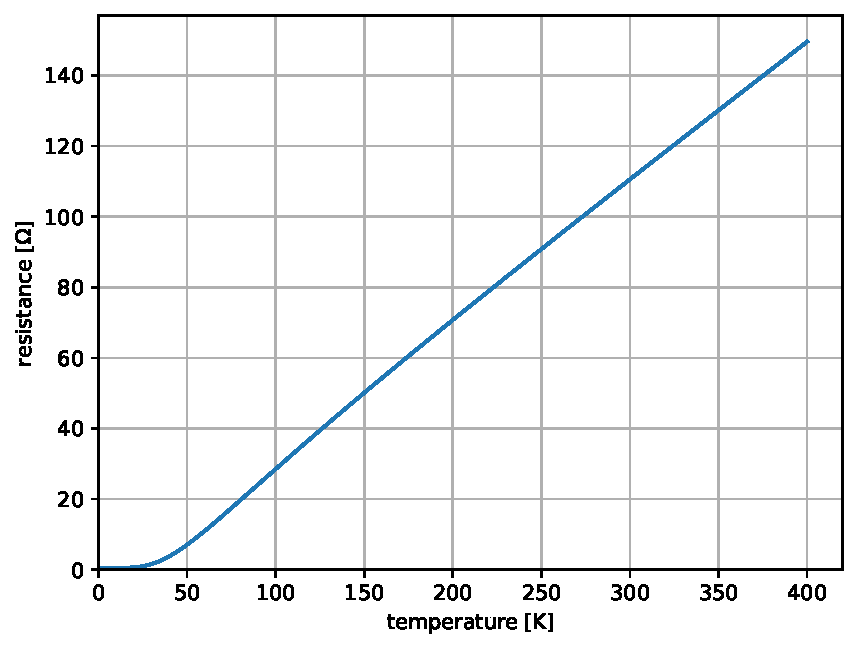
\includegraphics[width=10cm]{resistivity_Pt.pdf}
    \caption{白金の電気抵抗率の温度依存性}
    \label{rho_Pt}
\end{figure}
極低温領域に着目すると(図\ref{rho_Pt_low})、ある温度から立ち上がりはじめ、それまでは一定の値(残留抵抗)をとることが確認できる。
残留抵抗の値は$R_0 \sim 0.5 \,\Omega$である。
\begin{figure}[H]
    \centering
    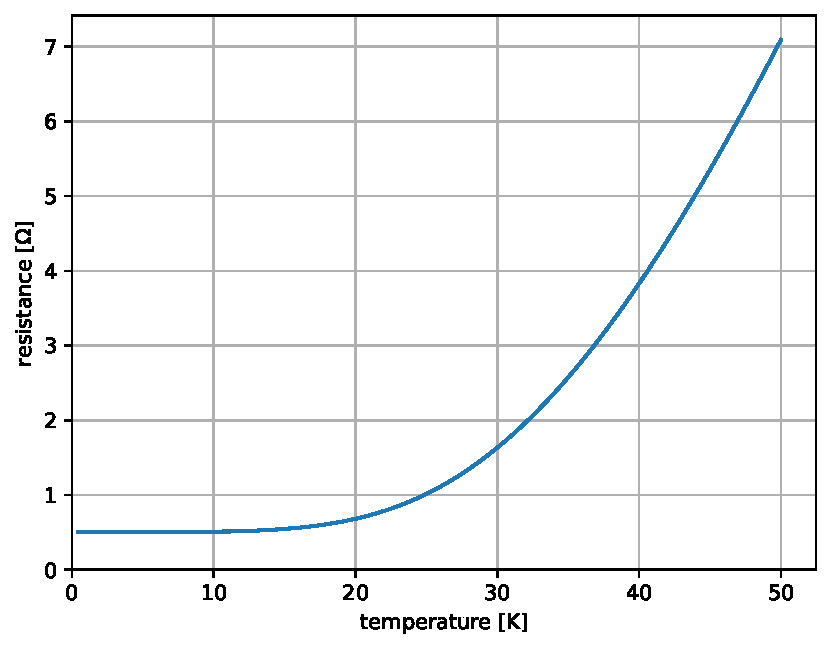
\includegraphics[width=10cm]{resistivity_Pt(lowtemp).pdf}
    \caption{白金の電気抵抗率の温度依存性(極低温領域)}
    \label{rho_Pt_low}
\end{figure}
%1.3
\subsection{半導体}
\subsubsection{真性半導体（課題3）}
真性半導体では、価電子帯から伝導帯に励起された電子と、価電子帯の励起電子の抜けた正孔が電気伝導に寄与する。
電導体の電子数$n$と価電子帯の正孔数$p$は等しい。電子、正孔の移動度をそれぞれ$\mu_e,\, \mu_h$とすると、真性半導体の電気伝導度$\sigma$は、
\begin{equation}
  \sigma = n e \mu_e + p e \mu_h = ne (\mu_e + \mu_h)
  \label{sigma}
\end{equation}
となる。
真性半導体のキャリア数は温度に大きく依存する。\par
周期境界条件を課した体積$V$の結晶の、波数空間における1状態が占める体積は、
\begin{equation}
  \frac{(2\pi)^3}{V}
\end{equation}
である。よって、波数空間上の半径$k$、厚さ$dk$の球殻の単位体積あたりの状態数は、スピン縮退を含めて、
\begin{equation}
  \frac{dN}{V} = 2 \cdot \frac{4\pi k^2 dk}{(2\pi)^3} = \frac{k^2}{\pi^2}dk
\end{equation}
である。ここで、伝導帯と安定点のエネルギーと電子のエネルギーをそれぞれ$E_c,\, E_e$、電子の有効質量を$m_e^*$とすると、
\begin{equation}
  E_e = E_c + \frac{\hbar^2 k^2}{2m_e^*}
\end{equation}
であり、これを波数$k$について整理して、さらに$E_e$で微分すると、
\begin{align}
  k^2 & = \frac{2m_e^* (E_e - E_c)}{\hbar^2} \\
  \frac{dk}{dE_e} & = \frac{m_e^*}{\hbar^2 k}
\end{align}
となる。よって、電導体の状態密度$D_c(E_e)$は、
\begin{align}
  D_c(E_e) & = \frac{1}{V} \frac{dN}{dE_e} = \frac{1}{V} \frac{dN}{dk} \frac{dk}{dE} \\
  & = \frac{k^2}{\pi^2} \frac{m_e^*}{\hbar^2 k} \\
  & = \frac{1}{2\pi^2} \left( \frac{2m_e^*}{\hbar^2} \right)^{3/2} \sqrt{E_e - E_c}
\end{align}
有限温度$T$の下では電子はFermi-Dirac分布に従う。化学ポテンシャル$\mu$のもとでのエネルギー$E$の状態の占有確率は、逆温度$\beta$を用いて、
\begin{equation}
  f(E) = \frac{1}{e^{\beta(E-\mu)} + 1}
\end{equation}
である。よって、伝導帯の電子数$n$は
\begin{align}
  n & = \int_{E_c}^{\infty} f(E_e) D_c(E_e) dE_e \\
  & = \frac{1}{2\pi^2} \left( \frac{2m_e^*}{\hbar^2} \right)^{3/2} \int_{E_c}^{\infty} \frac{\sqrt{E_e - E_c}}{e^{\beta(E_e-\mu)} + 1} dE_e
\end{align}
で求められる。通常、真性半導体では化学ポテンシャルはバンドギャップ内にあり、
$\beta (E_e - \mu) \gg 1$が成り立つので、占有状態は、
\begin{equation}
  f(E_e) \simeq e^{-\beta(E_e - \mu)}
\end{equation}
と近似できる。$x^2 = E_e - E_c$と置換すると、
\begin{align}
  n & = \frac{1}{2\pi^2} \left( \frac{2m_e^*}{\hbar^2} \right)^{3/2} \cdot e^{-\beta(E_c - \mu)} \cdot 2 \int_{0}^{\infty} x^2 e^{-\beta x^2} dx \\
  & = \frac{1}{\pi^2} \left( \frac{2m_e^*}{\hbar^2} \right)^{3/2} \cdot e^{-\beta(E_c - \mu)} \cdot \left( - \frac{d}{d\beta} \frac{1}{2} \sqrt{ \frac{\pi}{\beta}} \right) \\
  & = 2 \left( \frac{m_e^*}{2\pi \hbar^2 \beta} \right)^{3/2} e^{-\beta(E_c - \mu)}
  \label{n}
\end{align}
を得る。\par
価電子帯の頂上のエネルギーと、正孔のエネルギーをそれぞれ$E_v,\, E_h$とする。
正孔についての分散関係は、
\begin{equation}
  E_h = E_v - \frac{\hbar^2 k^2}{2 m_h^*}
\end{equation}
と展開できるので、正孔の状態密度は、
\begin{equation}
  D_h(E_h) = \frac{1}{2\pi^2} \left( \frac{2m_h^*}{\hbar^2} \right)^{3/2} \sqrt{E_v - E_h}
\end{equation}
となる。
価電子帯の状態が電子に占有されていない確率は、
\begin{equation}
  1 - f(E_h) = \frac{1}{e^{\beta(\mu - E_h)} + 1}
\end{equation}
であるので$\beta(\mu - E_v) \gg 1$のもとで、
\begin{equation}
  1 - f(E_h) \simeq e^{-\beta(\mu - E_h)}
\end{equation}
と近似できる。電子の場合と同じ積分を計算すると、
\begin{align}
  p & = \int_{E_v}^{-\infty} (1 - f(E_h)) D_h(E_h) dE_h \\
  & = 2 \left( \frac{m_h^*}{2\pi \hbar^2 \beta} \right)^{3/2} e^{-\beta(\mu - E_v)}
  \label{p}
\end{align}
を得る。\par
式(\ref{n})、(\ref{p})より、バンドギャップを$E_g = E_c - E_v$とすると、
\begin{align}
  n = p & = \sqrt{np} = 2 \left( \frac{\sqrt{m_e^* m_h^*}}{2\pi\hbar^2\beta} \right)^{3/2} \exp \left( -\frac{\beta E_g}{2} \right) \\
  & = 2 \left( \frac{k_B T}{2\pi\hbar^2} \right)^{3/2} \left( m_e^* m_h^* \right)^{3/4} \exp \left( - \frac{E_g}{2k_B T}\right) \\
  & = CT^{3/2} \exp \left( - \frac{E_g}{2k_B T}\right)
\end{align}
となる。また$\log n = \log p$より、化学ポテンシャル$\mu$すなわちFermi準位は、
\begin{equation}
  \mu = \frac{E_c + E_v}{2} + \frac{3}{4} k_B T \log \left(\frac{m_h^*}{m_e^*}\right)
\end{equation}
となる。よって、$\log \left(m_h^*/m_e^*\right) \sim 1$程度ならばFermi準位はバンドギャップの間に収まることがわかる。
式(\ref{sigma})より電気伝導度$\sigma$は、
\begin{align}
  \sigma & = e(\mu_e + \mu_h)CT^{3/2} \exp \left( - \frac{E_g}{2k_B T}\right) \\
  & \equiv \sigma_0 \exp \left( - \frac{E_g}{2k_B T}\right)
\end{align}
で得られる。$\sigma_0$の温度変化は指数部分に比べれば小さいので、両辺の対数をとれば、
\begin{equation}
  \log \sigma = \log \sigma_0 - \frac{E_g}{2k_B T}
\end{equation}
となり、狭い温度範囲では$\log \sigma_0$は定数とみなせる。すなわち縦軸$\log \sigma$と横軸$1/T$で描いたグラフは直線になりその傾きから$E_g$が求まる。
%1.2.2-2
\subsubsection{不純物半導体}
%1.2.3
\subsection{超伝導体}

\clearpage
\section{測定原理}
\subsection{電気抵抗の測定（課題7）}
\begin{wrapfigure}{r}{0.3\textwidth}
  \centering
  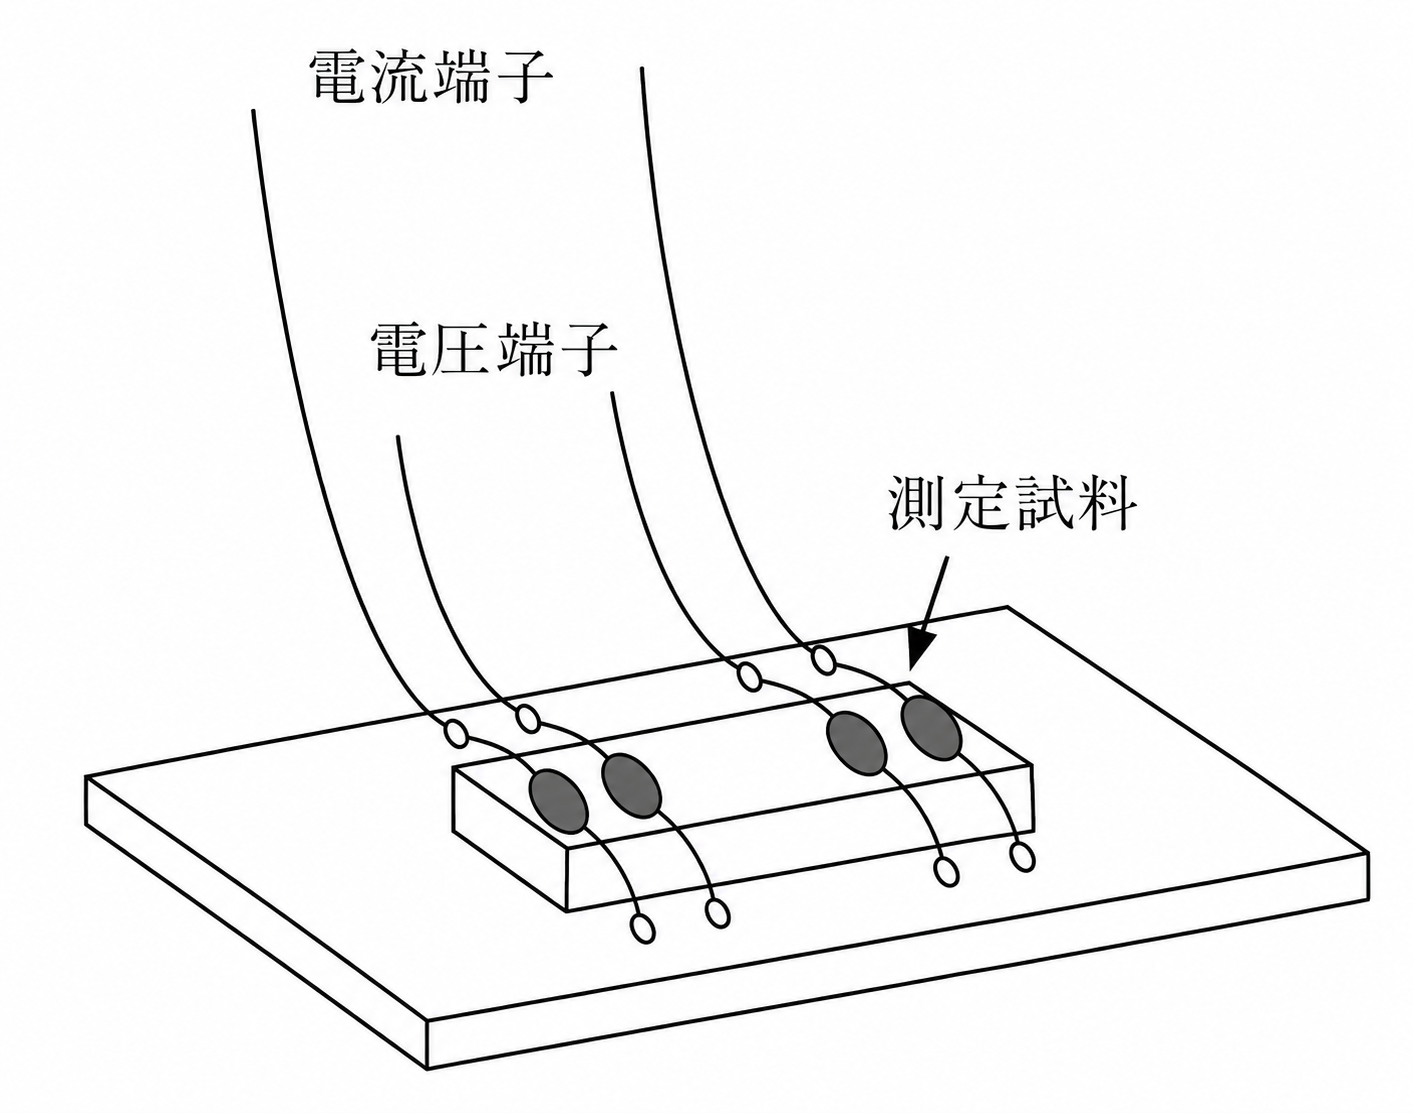
\includegraphics[width=\linewidth]{4tansi.png}
  \caption{直流四端子法}
  \label{4tansi-fig}
\end{wrapfigure}
金属の電気抵抗は一般に非常に小さく、テスターのような二端子法では導線の抵抗や端子の接触抵抗も測定することになってしまい、試料の抵抗を正確に測定できない。
そこで、正確な測定を行うために直流四端子法で測定を行う。図\ref{4tansi-fig}に直流四端子法の試料への接続の様子を示す。
実験で用いる高感度なデジタル電圧計の内部抵抗は一般に数$\mathrm{M}\Omega$〜数$\mathrm{G}\Omega$もあるので、接触端子と導線の抵抗を無視できる。
二端子法と四端子法を用いた測定系の等価回路を図\ref{circuit}に示す。
$r_i\,(i=1,2,3,4)$はそれぞれの端子の接触抵抗と導線抵抗の合成抵抗で、電流計と電圧計、試料の抵抗をそれぞれ$R_A,\,R_V,\,R$とする。
電源の起電力を$E$とし、回路に流れる電流を図$\ref{circuit}$のように定義する。
二端子回路における回路方程式は、
\begin{align}
  I & = I_1 + I_2
  \label{2tansi-EOC-1} \\
  I_2 R_V & = I_1 (R + r_1 + r_2)
  \label{2tansi-EOC-2}
\end{align}
となる。同様に四端子回路では、
\begin{align}
  I & = I_1 + I_2 
  \label{4tansi-EOC-1} \\
  I_1 R & = I_2 (R_V + r_3 + r_4)
  \label{4tansi-EOC-2}
\end{align}
である。電圧計の抵抗は非常に大きいので、
\begin{equation}
  \frac{R}{R_V},\,\frac{r_i}{R_V}, \ll 1 \,\, (i=1,2,3,4)
  \label{ll}
\end{equation}
が成り立つ。二端子法の測定抵抗$R_2^{ob}$は、
\begin{align}
  R_2^{ob} & = \frac{I_2 R_V}{I}
\end{align}
であるが、式(\ref{2tansi-EOC-1}-\ref{2tansi-EOC-2})より、
\begin{equation}
  I = I_2 \left( 1 + \frac{R_V}{R + r_1 + r_2}\right)
\end{equation}
であるので、
\begin{equation}
  R_2^{ob} = \frac{R_V}{1 + \dfrac{R_V}{R + r_1 + r_2}} \simeq R + r_1 + r_2
\end{equation}
となる。これから、二端子法では式(\ref{ll})の近似のもとでも、$r_1 + r_2$という余計な項がつき正確な測定が行えないことがわかる。
また二端子法の測定値の挙動は、接触抵抗の値に依存することがわかる。\par
四端子法の測定値$R_4^{ob}$は、
\begin{equation}
  R_4^{ob} = \frac{I_2 R_V}{I}
\end{equation}
である。式(\ref{4tansi-EOC-1}-\ref{4tansi-EOC-2})より、
\begin{equation}
  I = I_2 \left( 1 + \frac{R_V + r_3 + r_4}{R}\right)
\end{equation}
となるので、
\begin{equation}
  R_4^{ob} = \frac{R_V}{1 + \dfrac{R_V + r_3 + r_4}{R}} \simeq R
\end{equation}
を得る。これにより、四端子抵抗では式(\ref{ll})の0次近似のもとで正確に試料の抵抗を測れることがわかる。
\subsection{温度の測定}

\chapter{実験1（金属）}

\section{目的}
金属(銅)の電気抵抗の温度依存性を調べ、それらの特徴および原因について理解を深めるとともに電気抵抗測定法を学ぶ。
\section{測定手順}
\section{測定結果}


\chapter{実験2（半導体）}

\section{目的}
本実験では、最も典型的な半導体の一つであるゲルマニウム(Ge)を母体とした不純物半導体において電気伝導度の温度変化を測定し、その性質を物理的に理解する。
\section{測定手順}
\section{測定結果}

\chapter{実験3（超伝導体）}

\section{目的}
超伝導の基本的性質である完全導電性を電気抵抗測定により確認し、超伝導に対する理解を深める。
\section{測定手順}
\section{測定結果}


\begin{thebibliography}{99}
\bibitem{kyoukasho} 杉山清寛・福田光順・山中千博・下田正, (2025), 『[第6版]物理学実験』, 大阪大学出版会
\end{thebibliography}


\end{document}